%% ===================================================================
%%  TherapyTrace — IEEE conference paper
%%
%%  Compiles as-is on Overleaf: IEEEtran is part of the standard
%%  TeX Live installation there, so nothing needs to be uploaded for it.
%%  Do NOT add an IEEEtran.cls file to this project; a local copy would
%%  override Overleaf's and change the layout.
%%
%%  Build: pdfLaTeX -> BibTeX -> pdfLaTeX -> pdfLaTeX
%%  (Overleaf does this automatically; set the compiler to pdfLaTeX.)
%% ===================================================================
\documentclass[conference]{IEEEtran}
\IEEEoverridecommandlockouts

\usepackage{cite}
\usepackage{amsmath,amssymb,amsfonts}
\usepackage{algorithmic}
\usepackage{graphicx}
\usepackage{textcomp}
\usepackage{xcolor}
\usepackage{booktabs}
\usepackage{multirow}
\usepackage{url}

\def\BibTeX{{\rm B\kern-.05em{\sc i\kern-.025em b}\kern-.08em
    T\kern-.1667em\lower.7ex\hbox{E}\kern-.125emX}}

\begin{document}

\title{Measuring and Correcting Classifier Error Propagation\\
in a Longitudinal Psychotherapy Language Monitor}

\author{\IEEEauthorblockN{Nishant E S}
\IEEEauthorblockA{\textit{School of Computer Science and Engineering} \\
\textit{Vellore Institute of Technology}\\
Chennai, India \\
nishantelango77@gmail.com}
}

\maketitle

\begin{abstract}
Psychotherapy progress is assessed almost entirely through self-report
instruments administered weeks apart, while the language of the sessions
themselves leaves no quantitative trace. Computational work on therapy
transcripts has concentrated on classifying individual utterances, which is a
different question from the clinically relevant one of whether a person is
changing over time. We present TherapyTrace, a system that measures five
therapeutic process dimensions in client speech and normalises each session
against that client's own earlier sessions rather than against a population,
with James--Stein style shrinkage to stabilise small-sample variance. On
AnnoMI, a corpus of 133 expert-annotated motivational interviewing
demonstrations, we compare seven classifiers under conversation-grouped splits
and report a negative result: on the client talk-type task a paired $t$-test
cannot separate the best learner from any of the other six, and the spread
across all seven is smaller than the fold-to-fold variation of a single model.
This motivates our principal contribution. Rather than pursuing a stronger
classifier, we quantify how classification error propagates into the aggregate
a clinician would actually read. A classifier at $0.489$ macro-F1 yields a
session-level change-talk ratio biased upward by $0.25$; because the bias is
systematic it does not diminish with session length, and it compresses a true
range of $0.10$--$0.90$ into a displayed range of $0.63$--$0.85$. A prevalence
correction restores fidelity from a slope of $0.27$ to $0.80$. We show that the
textbook adjusted classify-and-count estimator clips at realistic session
lengths, pinning most sessions to the extremes, and adopt a Bayesian posterior
that remains in range by construction and supplies a credible interval. We
argue that measuring this propagation should be routine before any
model-derived aggregate is shown to a clinician.
\end{abstract}

\begin{IEEEkeywords}
clinical natural language processing, psychotherapy, motivational
interviewing, quantification learning, prevalence estimation, longitudinal
modelling, machine learning deployment
\end{IEEEkeywords}

% ===================================================================
\section{Introduction}

Psychotherapy is among the few clinical interventions whose primary medium is
language, and among the few whose progress is measured almost without
reference to it. A client attends weekly; every eight or twelve weeks an
instrument such as the PHQ-9 is administered, and the difference between two
administrations stands in for everything that occurred between them. The
speech that constitutes the treatment leaves no quantitative record.

Natural language processing is an obvious remedy, and a substantial literature
now applies it to therapy transcripts. Almost all of that work classifies
individual utterances: it asks what kind of thing a single sentence was. That
is a different question from the one a clinician asks, which is whether this
person is different from how they were a month ago. The unit of analysis in
the literature is the utterance; the unit of clinical interest is the person
over time.

A second gap is less often remarked upon. When an imperfect classifier is
embedded in a clinical interface, what the user sees is seldom a raw label. It
is an aggregate --- a rate, a proportion, a count --- computed over many
predictions. The relationship between the classifier's error and the bias of
that aggregate is rarely quantified, so a clinician may be shown a number whose
distortion is unknown to everyone involved.

\subsection{Contributions}

\begin{itemize}
\item A within-person scoring method for therapy transcripts that normalises
each session against the client's own earlier sessions, with shrinkage toward
a cohort prior so the index is reportable from the first sessions without
being unstable.
\item A seven-classifier comparison on AnnoMI under conversation-grouped
splits, establishing that the learners are statistically indistinguishable on
the client talk-type task and that the ceiling is set by the task rather than
the model.
\item A quantification of how that classifier's error propagates into the
session-level aggregate presented to the user: a systematic $+0.25$ bias that
does not diminish with more data, and a compression of the displayed range by
a factor of roughly three.
\item A correction, together with the finding that the standard algebraic
estimator fails at realistic session lengths and that a Bayesian posterior
does not.
\end{itemize}

% ===================================================================
\section{Related Work}

\subsection{Linguistic markers of psychological state}
Pennebaker et al. established that function words carry reliable information
about psychological state, with first-person singular pronoun use rising with
distress \cite{pennebaker2003}. Al-Mosaiwi and Johnstone showed that
absolutist vocabulary is elevated in anxiety, depression and suicidal
ideation by a larger margin than negative emotion words \cite{almosaiwi2018}.
Barrett et al. reviewed the evidence linking facial configuration to emotion
and found the mapping far weaker than applied work assumes
\cite{barrett2019}; we take this as a prohibition rather than a caveat and
emit no emotion inference from video.

Language has been modelled longitudinally, but outside the clinic. Tsakalidis
et al.\ identify ``moments of change'' in mood from sequences of a user's own
posts, distinguishing abrupt switches from gradual escalations and arguing for
temporally sensitive evaluation \cite{tsakalidis2022moments}. Successive
CLPsych shared tasks have built on that framing, from capturing moments of
change \cite{tsakalidis2022} to evidence of risk in online posts
\cite{chim2024} and, most recently, modelling self-state dynamics across whole
timelines \cite{tseriotou2025}. Matero et al.\ make the multi-level structure
explicit, separating within-person variation from between-person differences
in daily language about drinking \cite{matero2024} --- the same separation our
within-person normalisation performs, applied to a different substrate. That
substrate is the limitation we inherit from none of this work: social media
posts are frequent and self-authored. A course of therapy offers perhaps
twelve observations of dialogue, which is the regime this paper addresses.

\subsection{Process coding in motivational interviewing}
Motivational interviewing supplies the most developed process-coding
tradition, formalised in the MITI instrument \cite{moyers2016}. Automating it
is an established line of work: Flemotomos et al.\ score psychotherapy skills
from speech and language and report reliability against human coders
\cite{flemotomos2022}, Mehta et al.\ model several therapeutic approaches at
once rather than assuming a single modality \cite{mehta2022}, and Schmidt et
al.\ classify common factors and microcounseling skills \cite{schmidt2025}.
Session-level constructs beyond the code itself have also been formalised,
including linguistic synchrony between therapist and client
\cite{shapira2022} and therapist self-disclosure \cite{shapira2024}. The
relationship between codes and outcome is not simple: the meta-analysis of
Magill et al.\ over fifty-eight studies found no significant independent
association for raw change-talk frequency, a positive association between
sustain talk and \emph{worse} outcome ($r=0.19$), and an association between
the \emph{proportion} of change talk and reduced risk behaviour ($r=-0.16$)
\cite{magill2018}. The quantity worth computing is therefore a proportion, and
that is what our interface displays.

\subsection{Computational work on AnnoMI}
AnnoMI \cite{wu2022,wu2023} comprises 133 expert-annotated motivational
interviewing dialogues. It is important to state what the corpus is: these are
performed demonstrations used for MI training, not clinical recordings, and
23 transcripts are deliberately staged poor practice. Subsequent work includes
behaviour classification \cite{tavabi2021}, client motivational language for
psychotherapy agents \cite{hoang2024}, LLM-augmented corpus expansion with
bias measurement \cite{kumar2024}, multimodal multi-task context models
\cite{m3tcm2024}, and the use of AI-generated patient simulations to assess
sessions \cite{yosef2024}. Every one of these classifies,
generates or simulates a single utterance; none models the client as a subject
measured repeatedly. The same unit of analysis holds in the wider literature
on automated behavioural coding: Chen et al.\ transfer across corpora and
augment tasks to code psychotherapy conversations under low-resource
conditions \cite{chen2022lowresource}, and Pellemans et al.\ apply automated
MI coding to a chat-based suicide prevention helpline
\cite{pellemans2024} --- in both cases the object classified is the utterance.
A recent survey of large language models in psychotherapy reaches the same
conclusion across 69 studies, naming temporal modelling as an open direction
\cite{na2025survey}.

We note a methodological hazard. Reported figures on this corpus vary widely
and the split protocol is frequently unstated. Utterances within a
conversation share a speaker, a topic and a style, so an utterance-level split
permits a model to recognise a conversation it has memorised. Results obtained
under conversation-grouped splits are not directly comparable with results
whose protocol is unknown. The concern is not ours alone: Milintsevich et al.\
show that a widely used mental-health dataset supports far weaker conclusions
than its headline scores suggest once the data is examined rather than the
metric \cite{milintsevich2024}, and Shani and Stade argue that computational
mental-health research frequently reports numbers whose construct validity is
never established \cite{shani2025}. The present paper takes that argument one
step further: a quantity can be validly defined and still be displayed
wrongly, if the error of the classifier producing it is left unmeasured.

\subsection{Quantification and prevalence estimation}
Estimating class prevalence from the output of an imperfect classifier is
known as quantification \cite{forman2008}, now a developed subfield with a
dedicated monograph \cite{esuli2023}. Counting predicted labels is a biased
estimator; corrections include adjusting outputs for shifted priors
\cite{saerens2002} and adjusted classify-and-count. A recent comparison of
24 quantification algorithms over more than 40 datasets finds that no single
method dominates and that relative performance depends on sample size and the
degree of prior shift \cite{schumacher2025}, which is consistent with the
instability we observe for adjusted classify-and-count at the sample sizes a
single session provides. To our knowledge this machinery has not been applied
to the question of what a clinical dashboard should display, which is the gap
this paper addresses.

% ===================================================================
\section{Method}

\begin{figure*}[t]
\centering
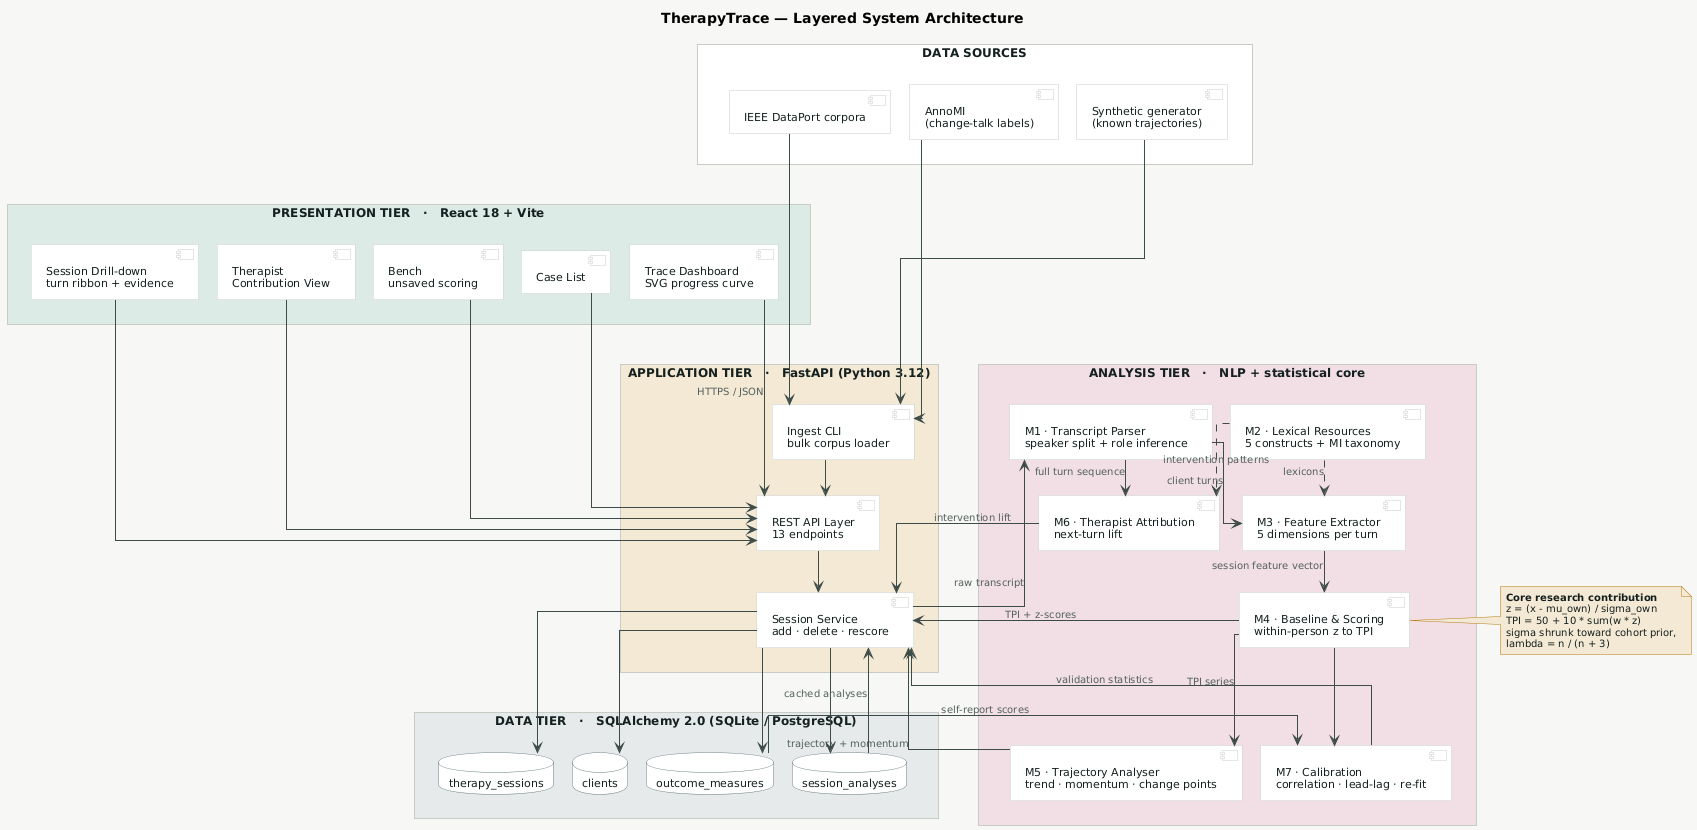
\includegraphics[width=0.84\textwidth]{figures/TherapyTrace_Architecture.png}
\caption{System architecture. The measurement layer is rule-based and
deterministic, so every score traces to specific phrases in the transcript.
The supervised layer is additive: the system functions without it. Optional
modalities enter as bounded modifiers rather than as primary signal.}
\label{fig:arch}
\end{figure*}

\subsection{Process dimensions}
Each client turn is scored on five dimensions chosen because therapy is
expected to move them and each is measurable from surface evidence:
self-agency, future orientation, emotional granularity, problem ownership and
reflection depth. Internal attribution counts as ownership only when it is not
self-blame; absolutist self-criticism is penalised rather than rewarded.
Session features aggregate turn scores weighted by $\sqrt{\text{word count}}$,
so a long narrative counts for more than an acknowledgement but not
proportionally more.

\subsection{Within-person normalisation}
The central commitment is that each session is scored against the client's own
earlier sessions. For dimension $d$ in session $s$,
\begin{equation}
z_d(s) = \frac{x_d(s) - \mu_d^{\text{own}}}{\sigma_d^{\text{own}}},
\end{equation}
and the index is a weighted sum centred at fifty,
\begin{equation}
\mathrm{TPI}(s) = 50 + 10 \sum_d w_d \, z_d(s).
\end{equation}
Fifty therefore denotes this person speaking as this person usually speaks.

\subsection{Shrinkage}
A standard deviation estimated from two or three sessions is unstable, and an
unstable denominator produces erratic indices. We shrink the client's own
deviation toward a cohort prior,
\begin{equation}
\sigma^{\text{pooled}}_d = \lambda \sigma^{\text{own}}_d
  + (1-\lambda)\sigma^{\text{cohort}}_d, \quad
\lambda = \frac{n}{n + k_0},
\end{equation}
with $k_0 = 3$. Early in a case the estimate leans on the prior; by eight to
ten sessions it is dominated by the client's own variability.

\subsection{Supervised layer}
Two classifiers are trained on AnnoMI: client talk type (change, sustain,
neutral) and therapist behaviour (question, reflection, therapist input,
other). The session-level quantity the interface displays is
\begin{equation}
r = \frac{n_{\text{change}}}{n_{\text{change}} + n_{\text{sustain}}},
\end{equation}
over directional turns, following \cite{magill2018}.

\subsection{Error propagation}
Let $M$ be the misclassification matrix restricted to the directional classes,
with $M_{ij} = P(\hat{y}=j \mid y=i)$. If the true directional prevalence is
$p$, the classifier predicts change with probability
\begin{equation}
\theta(p) = p\,M_{cc} + (1-p)\,M_{sc}.
\label{eq:theta}
\end{equation}
Counting predictions and dividing estimates $\theta(p)$, not $p$. The two
coincide only when $M$ is the identity, so the naive ratio is biased for any
imperfect classifier, and the bias is systematic: it does not vanish as the
number of turns grows.

\subsection{Correction}
Adjusted classify-and-count inverts \eqref{eq:theta} algebraically. We find
this fails in practice at the session lengths that occur (Section
\ref{sec:correction}), and instead treat the observed count as binomial in
$\theta(p)$ and compute a posterior over $p$ under a flat prior:
\begin{equation}
P(p \mid n_c, n_s) \propto \theta(p)^{n_c}\,\bigl(1-\theta(p)\bigr)^{n_s}.
\end{equation}
The posterior mean lies in $[0,1]$ by construction, shrinks toward the centre
when evidence is thin, and yields a credible interval that the interface
displays alongside the point estimate.

% ===================================================================
\section{Experimental Setup}

\textbf{Data.} AnnoMI \cite{wu2023}: 133 conversations, 9{,}699 unique
utterances. After filtering turns shorter than three words, the client task
has 4{,}740 utterances and the therapist task 5{,}078.

\textbf{Protocol.} Splits are grouped by transcript identifier and never by
utterance. Twenty-five per cent of conversations are held out before any model
is fitted; selection runs as five-fold \texttt{GroupKFold} over the remainder;
the held-out conversations are scored once, for every model.

\textbf{Features.} Every learner sees an identical matrix: TF-IDF word
unigrams and bigrams, character 3--5 grams, and twelve lexicon features. A
difference in score is therefore attributable to the learner alone.

\textbf{Class balancing.} The client corpus is 53\% neutral, so a learner
optimising raw accuracy under-predicts minority classes for reasons unrelated
to the algorithm. Every model is balanced by whatever mechanism it offers:
class weights for linear models and LightGBM, balanced subsampling for the
forest, uniform priors for naive Bayes, injected per-row weights for XGBoost.
The MLP cannot be balanced in scikit-learn; we report this asymmetry rather
than conceal it.

% ===================================================================
\section{Results}

\subsection{Model comparison}

\begin{table}[t]
\caption{Client talk type, held-out conversations ($n=1{,}656$ utterances
from 34 unseen conversations). $p$ is a paired $t$-test against the
selected model across the five CV folds.}
\label{tab:client}
\centering
\footnotesize
\begin{tabular}{lcccc}
\toprule
Model & CV macro-F1 & Acc. & Macro-F1 & $p$ \\
\midrule
Majority class       & $0.228$ & $0.554$ & $0.238$ & --- \\
Naive Bayes          & $\mathbf{0.465}$ & $0.525$ & $0.457$ & --- \\
Logistic Regression  & $0.464$ & $0.542$ & $0.489$ & $0.938$ \\
Linear SVM           & $0.459$ & $0.566$ & $0.492$ & $0.741$ \\
Random Forest        & $0.420$ & $0.614$ & $\mathbf{0.500}$ & $0.068$ \\
XGBoost              & $0.463$ & $0.549$ & $0.485$ & $0.880$ \\
LightGBM             & $0.424$ & $0.541$ & $0.425$ & $0.092$ \\
MLP (128 hidden)     & $0.414$ & $\mathbf{0.618}$ & $0.462$ & $0.264$ \\
\bottomrule
\end{tabular}
\end{table}

\begin{table}[t]
\caption{Therapist behaviour, held-out conversations ($n=1{,}794$).}
\label{tab:therapist}
\centering
\footnotesize
\begin{tabular}{lcccc}
\toprule
Model & CV macro-F1 & Acc. & Macro-F1 & $p$ \\
\midrule
Majority class       & $0.145$ & $0.304$ & $0.117$ & --- \\
Naive Bayes          & $0.585$ & $0.650$ & $0.598$ & $0.011$ \\
Logistic Regression  & $\mathbf{0.639}$ & $0.664$ & $0.608$ & --- \\
Linear SVM           & $0.627$ & $0.678$ & $0.612$ & $0.115$ \\
Random Forest        & $0.584$ & $0.643$ & $0.600$ & $0.009$ \\
XGBoost              & $0.625$ & $\mathbf{0.688}$ & $\mathbf{0.651}$ & $0.127$ \\
LightGBM             & $0.629$ & $0.687$ & $0.630$ & $0.244$ \\
MLP (128 hidden)     & $0.613$ & $0.684$ & $0.620$ & $0.015$ \\
\bottomrule
\end{tabular}
\end{table}

Tables \ref{tab:client} and \ref{tab:therapist} report all seven learners and
the majority-class floor. Three observations follow.

First, accuracy is uninformative on the client task. The majority-class floor
is $0.554$, higher than any real learner achieves; a model answering
``neutral'' throughout outscores all seven. The metric that moves is macro-F1,
rising from $0.238$ at the floor to $0.489$. The MLP illustrates the hazard
sharply: it records the highest accuracy ($0.618$) and the lowest sustain-class
F1 ($0.131$), achieving the former by predicting the majority class.

Second, the learners are statistically indistinguishable on the client task.
The smallest $p$-value against any competitor is $0.068$. The spread between
best and worst of the seven is $0.051$ macro-F1 against a fold-to-fold
standard deviation of $0.043$ for a single model: the differences lie inside
the noise.

Third, cost does not buy accuracy. Measured on an idle machine, XGBoost
requires $56.0$\,s to fit on the client task where naive Bayes requires
$0.01$\,s --- three orders of magnitude for no gain.

\subsection{Per-class behaviour and the deployment criterion}

\begin{table}[t]
\caption{Client talk type: per-class recall. Sustain is the weak class for
every learner, and varies almost five-fold across them.}
\label{tab:recall}
\centering
\footnotesize
\begin{tabular}{lccc}
\toprule
Model & change & neutral & sustain \\
\midrule
Naive Bayes          & $0.617$ & $0.580$ & $0.210$ \\
Logistic Regression  & $0.534$ & $0.612$ & $\mathbf{0.335}$ \\
Linear SVM           & $0.499$ & $0.687$ & $0.290$ \\
Random Forest        & $0.581$ & $0.773$ & $0.159$ \\
XGBoost              & $0.570$ & $0.626$ & $0.276$ \\
LightGBM             & $0.472$ & $0.709$ & $0.117$ \\
MLP (128 hidden)     & $0.517$ & $\mathbf{0.841}$ & $0.072$ \\
\bottomrule
\end{tabular}
\end{table}

Table \ref{tab:recall} shows what the averages conceal. Sustain recall ranges
from $0.072$ to $0.335$, and the model selected by macro-F1 sits near the
bottom of that range. Because the displayed quantity depends on separating
change from sustain, sustain recall rather than macro-F1 is the correct
deployment criterion --- a conclusion that selects logistic regression.

\subsection{Error propagation}

\begin{figure*}[t]
\centering
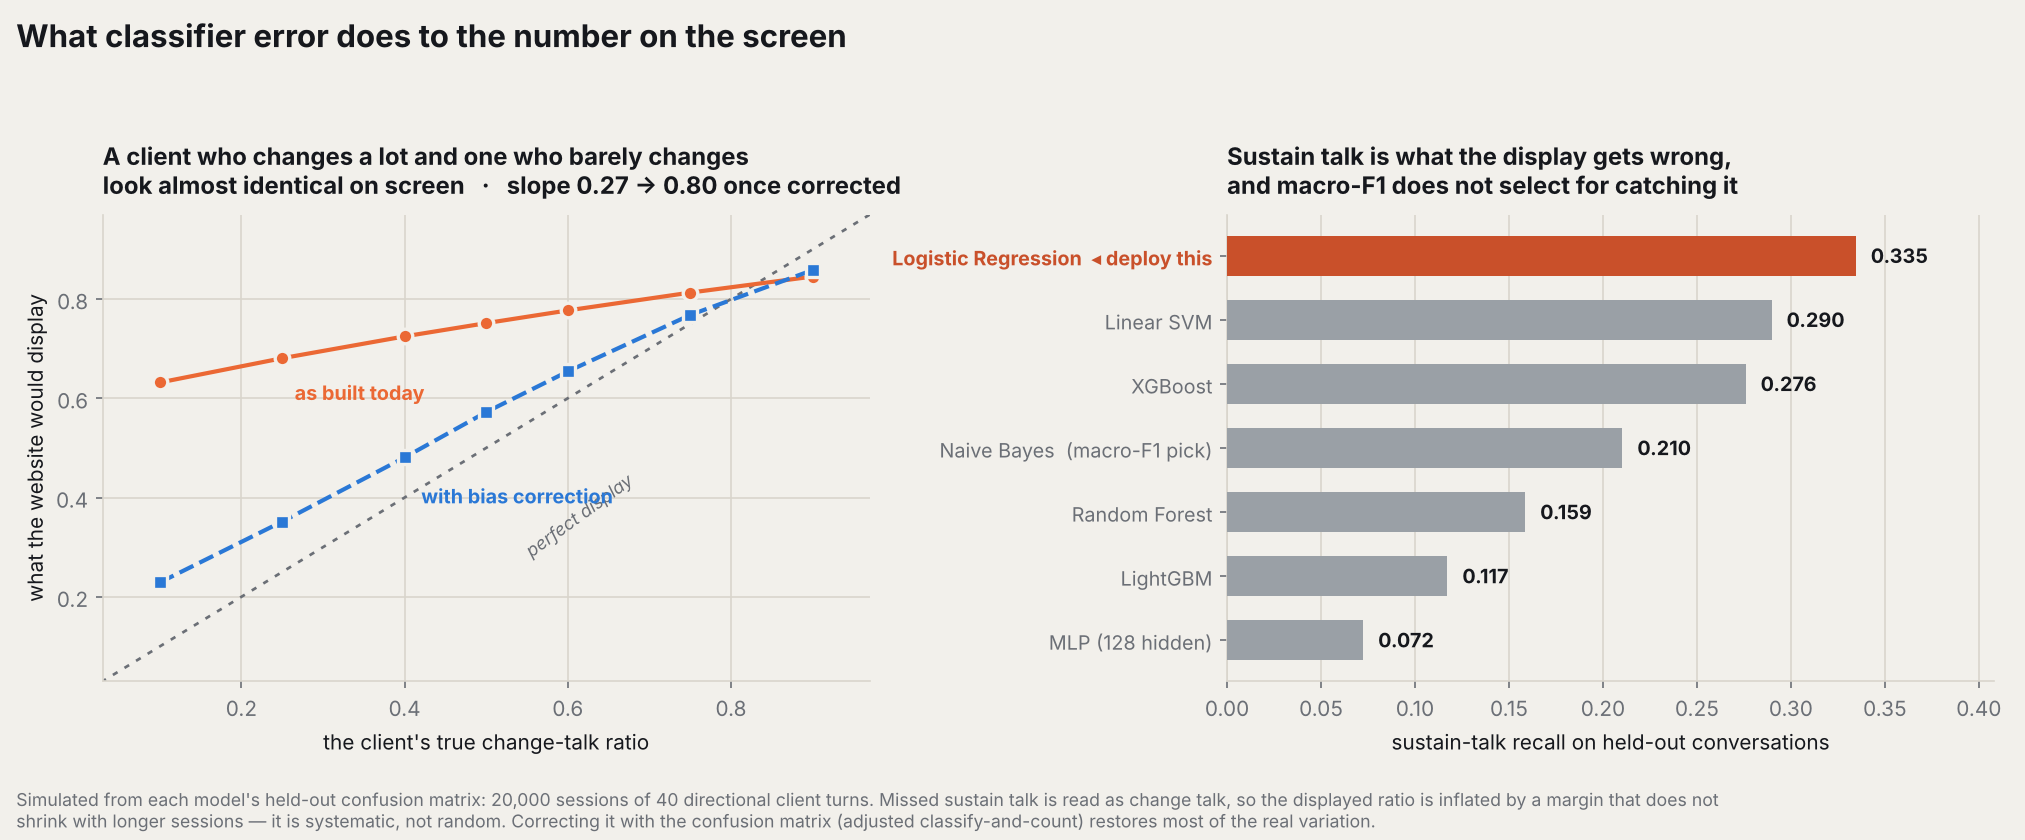
\includegraphics[width=0.92\textwidth]{figures/bench_reliability.png}
\caption{Left: the ratio the interface would display against the client's true
ratio, with and without correction; the dotted diagonal marks a faithful
display. Uncorrected, a true range of $0.10$--$0.90$ is compressed to
$0.63$--$0.85$. Right: sustain recall by learner, which drives the bias.
Simulated from each model's held-out confusion matrix over 20{,}000 sessions
of 40 directional turns.}
\label{fig:reliability}
\end{figure*}

A macro-F1 of $0.489$ does not answer whether the number on the screen can be
trusted. We simulated 20{,}000 sessions of 40 directional turns, corrupting
each turn according to the deployed model's held-out confusion matrix.

For a client genuinely evenly split between change and sustain talk, the
uncorrected interface displays $0.75$. The bias of $+0.25$ does not diminish
with session length: $0.752$ at ten directional turns and $0.752$ at one
hundred and twenty. It is systematic, and more data does not help.

The cause is specific. Sustain talk is recovered as sustain only $21\%$ of the
time and read as change $31\%$ of the time; missed sustain inflates the
numerator and shrinks the denominator at once, and both errors push the ratio
the same way.

The consequence is more serious than the bias. As Fig.~\ref{fig:reliability}
shows, a true range of $0.10$--$0.90$ compresses to a displayed range of
$0.63$--$0.85$, a slope of $0.27$. A client barely changing and one changing a
great deal appear nearly identical --- precisely the comparison the system
exists to support.

\subsection{Correction}
\label{sec:correction}

Applying the correction of Section III-F restores the slope from $0.27$ to
$0.80$ and reduces the midpoint bias from $+0.25$ to $+0.07$. Variance rises,
which is the honest trade: the estimate becomes noisier but ceases to be
systematically wrong in one direction.

We emphasise a practical finding. Adjusted classify-and-count, the textbook
correction, was implemented first. It is adequate on long sequences, but the
sessions here carry seven to fifteen directional turns, and at that size the
algebraic solve lands outside $[0,1]$ and must be clamped: eight of twelve
demonstration sessions pinned to exactly $0.00$ or $1.00$, producing a step
function between two extremes asserted with total confidence. That is a worse
failure than the bias it removes. The Bayesian posterior avoids it by
construction. This was discovered by running the estimator on data rather than
by reasoning about it, and we report it because the failure mode is not
apparent from the estimator's definition.

Even corrected, a session-to-session change of $+0.10$ moves the display in
the correct direction only about $58\%$ of the time at forty turns, against
$50\%$ for a coin. The series supports a trend across several sessions and does
not support a judgement about a single pair, and the interface says so.

\subsection{Reframing the task}

\begin{table}[t]
\caption{Three-class against binary change-versus-sustain framing, identical
protocol, deployed model.}
\label{tab:binary}
\centering
\footnotesize
\begin{tabular}{lccc}
\toprule
Metric & Three-class & Binary & $\Delta$ \\
\midrule
Accuracy        & $0.542$ & $0.653$ & $+0.111$ \\
Macro-F1        & $0.489$ & $0.616$ & $+0.127$ \\
Sustain F1      & $0.351$ & $0.497$ & $+0.145$ \\
Sustain recall  & $0.335$ & $0.478$ & $+0.143$ \\
ROC-AUC         & $0.678$ & $0.660$ & $-0.018$ \\
\bottomrule
\end{tabular}
\end{table}

Because the interface never uses the neutral class, the three-class problem is
not the problem the product needs solved. Table \ref{tab:binary} evaluates a
binary change-versus-sustain classifier on the 2{,}211 directional turns under
the identical protocol. Sustain recall rises from $0.335$ to $0.478$, which
directly reduces the display bias.

Two limits are stated. Accuracy clears its own floor of $0.644$ by only
$0.009$; macro-F1 clears its floor by $0.225$, and that is the real margin.
And the binary figures assume the directional turns are already identified,
which holds for an annotated corpus and not in deployment: realising this gain
requires a two-stage model whose first stage contributes its own error.

\subsection{State-conditional response}

\begin{table}[t]
\caption{Probability of change talk following each therapist move, by the
client's state beforehand. 1{,}815 triples across 123 conversations.}
\label{tab:state}
\centering
\footnotesize
\begin{tabular}{lcccc}
\toprule
Therapist move & Stuck & Middling & Moving & $p$ \\
\midrule
Question         & $0.268$ & $0.412$ & $0.479$ & $<0.001$ \\
Reflection       & $0.260$ & $0.382$ & $0.455$ & $0.001$ \\
Therapist input  & $0.253$ & $0.265$ & $0.296$ & n.s. \\
Other            & $0.244$ & $0.331$ & $0.415$ & --- \\
\bottomrule
\end{tabular}
\end{table}

Table \ref{tab:state} shows that the association between a therapist move and
subsequent change talk depends strongly on the client's state beforehand.
Questions and reflections roughly double their association when the client is
already moving; therapist input shows almost no state dependence.

The interpretive caution is essential: these are associations, not causal
effects. A client already moving produces more change talk whatever the
therapist does, so part of the difference is confounding by indication. What
the analysis supports is the weaker claim that an unconditional average ---
questions are followed by change talk $0.369$ of the time --- averages over two
very different situations and is the wrong number to act on.

% ===================================================================
\section{Discussion}

The results support a conclusion that is unusual to report. The classification
component of this system is mediocre, cannot readily be improved by changing
the learner, and this does not undermine the work, because classification was
never the contribution.

What the results establish is that an imperfect classifier can still support a
usable session-level clinical measure, provided the error it induces in the
aggregate is measured and corrected. Without correction the system would have
displayed a confidently wrong number: $0.75$ for a client who was evenly split,
with real differences between clients compressed into near-invisibility. That
failure was identified before deployment by measuring it.

We suggest this should be routine. Where a model-derived aggregate is shown to
a clinician, the propagation from per-item error to displayed quantity is
computable from a held-out confusion matrix and takes little effort. It is not,
at present, commonly reported.

% ===================================================================
\section{Limitations}

The central claim concerns change within a person across sessions, and no
public corpus contains repeated sessions from the same client; that layer is
demonstrated on synthetic cases with known trajectories, which is pipeline
validation and not clinical evidence. AnnoMI consists of performed
demonstrations, so transfer to genuine sessions is unmeasured. The deployed
classifier reaches $0.489$ macro-F1 and single-session judgements are not
supported even after correction. The MLP alone could not be class-balanced. No
fine-tuned transformer baseline was run. The lexicons and models are
English-specific.

% ===================================================================
\section{Conclusion}

We presented a system that measures therapeutic process within a client across
sessions rather than classifying utterances in isolation, and showed on AnnoMI
that seven classifiers are statistically indistinguishable on the client
talk-type task. Taking that as evidence against pursuing a stronger
classifier, we instead measured how classification error reaches the user: a
systematic $+0.25$ bias in the displayed ratio that does not diminish with
more data and compresses the displayed range threefold. A prevalence
correction restores fidelity from a slope of $0.27$ to $0.80$, and we showed
that the standard algebraic estimator fails at realistic session lengths while
a Bayesian posterior does not.

Future work is to obtain a longitudinal clinical corpus under ethics approval,
add a transformer tier, and build the two-stage directional classifier so the
binary gain can reach deployment.

% ===================================================================
\bibliographystyle{IEEEtran}
\bibliography{refs}

\end{document}
